\section{Описание процесса проектирования ПК}



\subsection{Описание вариантов использования ПК}

Проектирование программного комплекса начинается с прояснения функциональных
требований из технического задания. В итоге появляется развернутый и
детализированный список требований, характеризующих процессы в текущей
предметной области.  Распространенными способами такого описания являются
UML-диаграммы прецедентов (use case) и пользовательские истории (user story).

UML-диаграмма прецедентов состоит из набора сценариев взаимодействия программы
с внешней средой в соответствии с требованиями. Прецеденты описываются от лица
некоторых внешних сущностей, называемых акторами. Акторы взаимодействуют с
системой, меняют ее для достижения своих целей. Между актерами и прецедентами
устанавливаются направленные соединения --- связи коммуникации, которые также
снабжаются информацией об участвующих данных и кратности соединения.

Прецеденты могут образовывать структуру с помощью вида связи, который
называется связью использования. Таким образом, появляются группы прецедентов,
исполняемых вместе. Для демонстрации родственных отношений между прецедентами
используется связь расширения.

Другим похожим способом описания вариантов использования приложений являются
пользовательские истории, получившие широкое распространение как составные
части многих гибких методологий разработки (SCRUM, экстремальное
программирование и другие). Основная суть заключается в выделении сущности
пользователя и написании от его лица особых фраз по специальному шаблону,
которые показывают сценарии работы системы и их применение в контексте бизнес
задач. Воспользуемся следующим шаблоном:

\hspace{2cm}\textit{
    Я как <\uline{роль}> хочу <\uline{возможность}>, чтобы
    <\uline{цель}>.
}


Главным отличием от use case является то, что пользовательские истории намного
ближе к обычному клиенту, не обладающему профессиональными навыками разработки
ПО, и формулируются на повседневном языке, отчего, однако, не оказываются столь
подробными как UML-диаграммы прецедентов.

В Pharmacy Console присутствуют такие акторы, как администратор аптеки,
бухгалтер аптеки и база данных. Напишем сначала пользовательские истории для
администратора и бухгалтера, а затем построим диаграмму прецедентов.

Пользовательские истории:
\begin{itemize}
    \item я как администратор аптеки хочу иметь возможность добавлять сведения
        о лекарствах, чтобы вести их учет;
    \item я как администратор аптеки хочу иметь возможность добавлять к
        лекарствам список болезней, которые те лечат, чтобы консультировать
        клиентов аптеки;
    \item я как администратор аптеки хочу иметь возможность удалять лекарства
        и болезни (если нет связи с лекарствами), чтобы легко обновлять
        ассортимент аптеки;
    \item я как администратор аптеки хочу иметь возможность редактировать
        информацию о лекарствах и болезнях, чтобы использовать это при
        обновлении ассортимента и новых поставках;
    \item я как администратор аптеки хочу иметь возможность видеть списки всех
        лекарств и болезней в виде таблицы, чтобы легко находить о них
        информацию;
    \item я как администратор аптеки хочу иметь возможность фильтровать
        отображаемый список лекарств по болезням, которые те лечат, чтобы легко
        консультировать клиентов;
    \item я как администратор аптеки хочу иметь возможность создавать новый
        заказы, указывая число покупаемых товаров, с автоматическим подсчетом
        суммы заказов;
    \item я как администратор аптеки хочу видеть список всех заказов (с
        возможностью указания периода времени) и общую сумму этих заказов.
    \item я как бухгалтер аптеки, хочу иметь возможность получать отчет по
        совершенным заказам в определенный период в формате PDF, чтобы
        совершать бухгалтерский учет;
\end{itemize}

Диаграмма прецедентов изображена на рис. \ref{pic:use-case-dia}.

\addimghere{res/design/use-case-d.png}{1}
{Диаграмма прецедентов программы}{pic:use-case-dia}

\addimghere{res/design/ui-proto.png}{1}{Прототип дизайна приложения}{pic:ui-proto}


\subsection{Создание прототипа интерфейса пользователя}

На основе проработанные прецеденты теперь можно описать процессы в терминах
пользовательских интерфейсов, детализировав тем самым реализацию. Прецеденты
удобно разбить на отдельные экранные формы и определить содержимое графических
представлений, способы их взаимодействия. То есть, для каждой формы можно
привести набор графических элементов, действия пользователя и отклики системы.
Полученные перечни удобно свести в таблицы экранных форм (табл. 1.1, 1.2, 1.3).
Здесь не приводятся таблицы для окон <<Добавление/редактирование заболеваний>>,
<<Создание заказа>> и вкладок <<Болезни>>, <<Заказы>>, так как они тривиальны и
выполняются аналогично.

Кроме того, общий дизайн всей программы был вначале прототипирован с помощью
сервиса Figma (рис. \ref{pic:ui-proto}).


\subsection{Разработка объектной модели}

На этом этапе можно перейти к проектированию объектной модели, отображающую
основные понятия предметной области и их взаимосвязь как совокупность типов
объектов (далее классов, но следует отличать их от классов в языках
программирования). Модель строится на основе анализа предметной области задачи.

В UML объектная модель представляется в виде диаграммы классов (class diagram),
которая состоит из собственно классов, содержащих атрибуты (свойства сущности)
и операции (поведения сущностей). Между собой классы выстраивают ассоциации,
показывающие семантический смысл отношения двух сущностей. Ассоциации могут иметь
кратность. Особый интерес представляют ассоциации, которые отражают структурные
отношения (<<содержит>>, <<включает>>, <<хранит>>, и т.д.).

С точки зрения предметной области легко видеть, что Pharmacy Console имеет
сущности <<Лекарство>>, <<Заболевание>> и <<Заказ лекарства>>. На рис.
\ref{pic:entity-dia} отображены данные классы с атрибутами и операциями.
Детальное описание операций в данном случае не требуется.

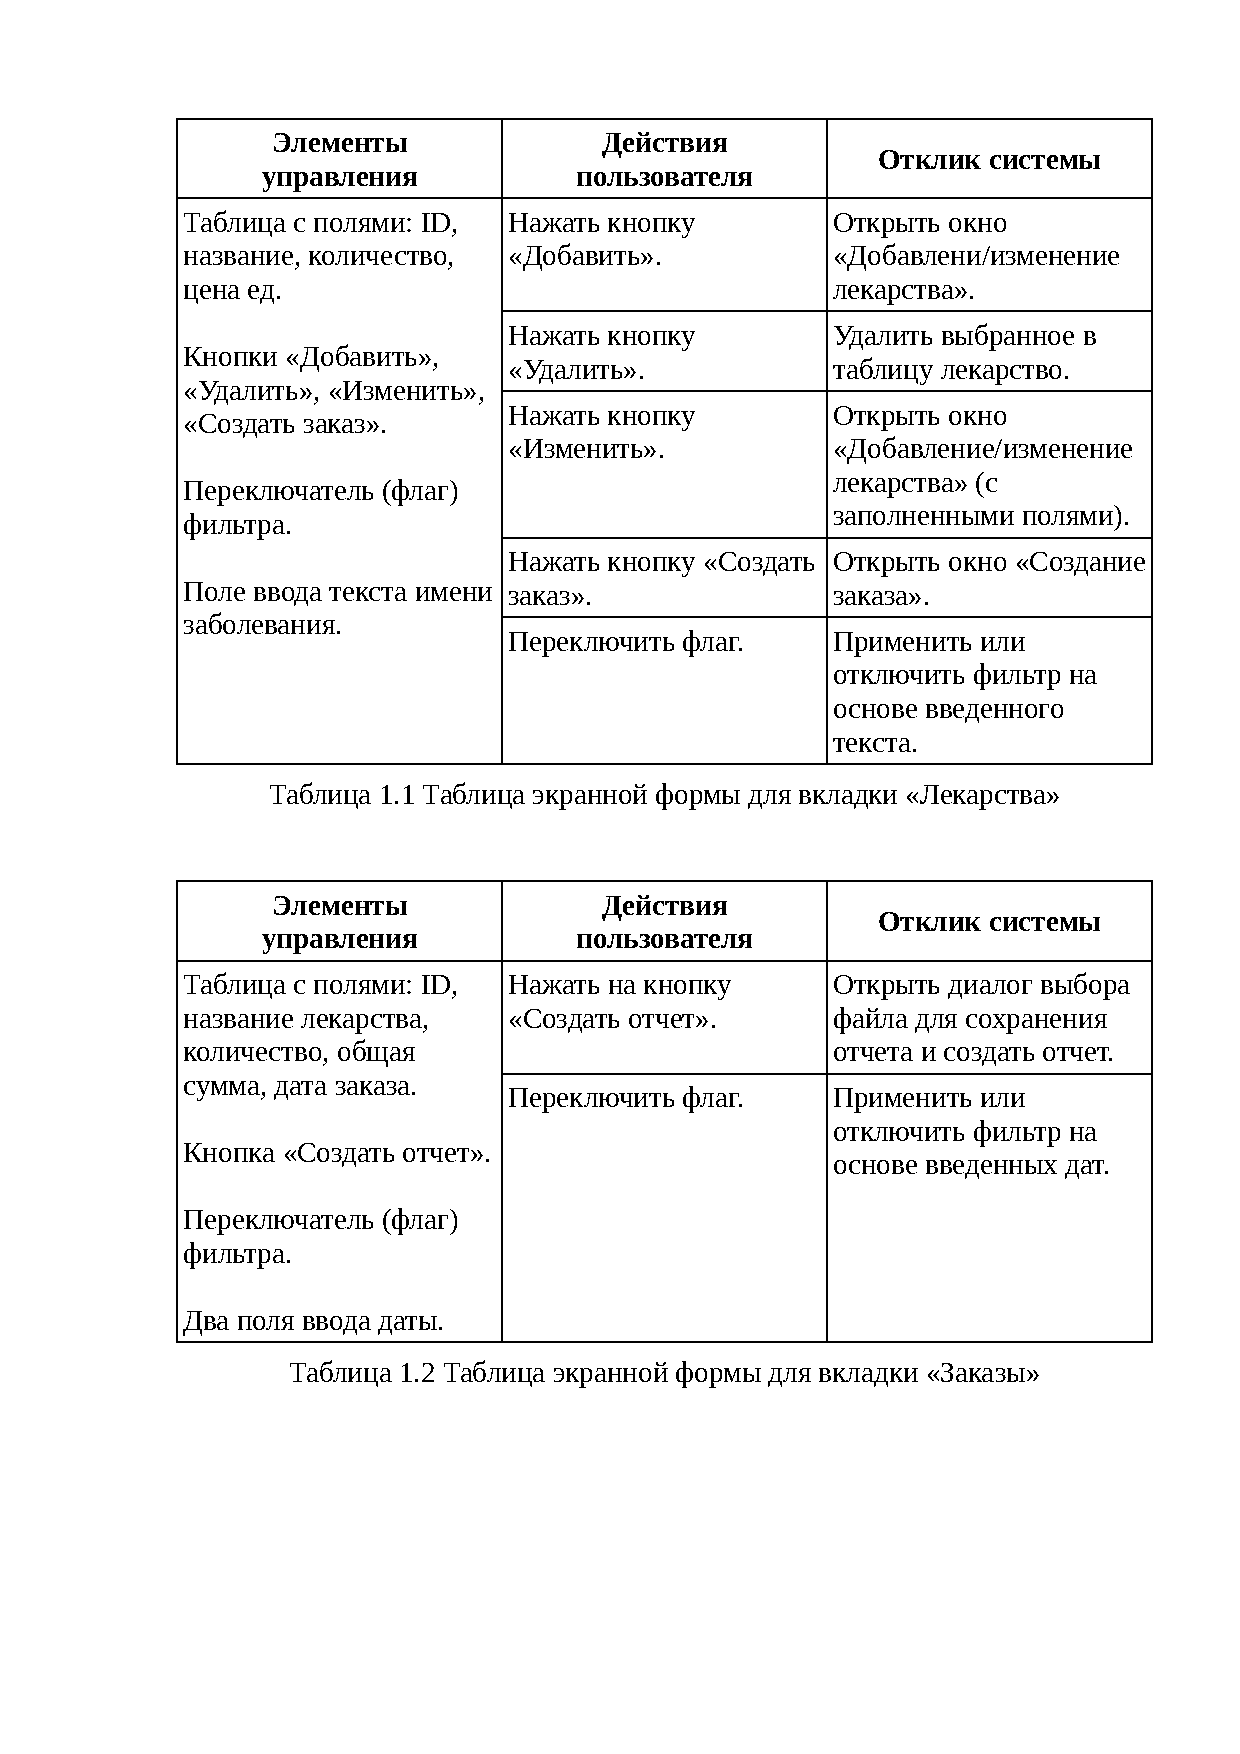
\includepdf[pages=1,pagecommand={}]{res/design/forms.pdf}
\begin{minipage}[t][6.5cm]{1\linewidth}
    \includepdf[pages=2,pagecommand={}]{res/design/forms.pdf}
\end{minipage}

\addimghere{res/design/entity-d.png}{0.7}
{Диаграмма сущностей}{pic:entity-dia}

\subsection{Построение диаграммы программных классов}


Получив объектную модель программы, можно перейти к спецификации программной
реализации этой модели на основе программных классов и интерфейсов. Диаграмма
классов является расширением диаграммы сущностей и добавляет в нее новые
смыслы, важные при реализации структуры на объектно-ориентированном языке
программирования: новые атрибуты, операции, связи, конкретизируется тип связи
(ассоциация, агрегация, наследование).

На рис. \ref{pic:class-dia} изображена UML-диаграмма классов. Заметим, что тут
появились некоторые новые классы: DAO, сервисы и контроллеры. На данном рисунке
также приведен лишь фрагмент полной диаграммы классов из-за большой сложности
последней.

\addimg{res/design/class-d.png}{1}{Диаграмма классов}{pic:class-dia}


\subsection{Описание поведения ПК}


Перед тем, как переходить к непосредственной реализации кода, необходимо еще
определить поведение программы без конкретизации механизмов их реализации. В
этом качестве используется диаграмма последовательностей (sequence diagram).

Диаграмма показывает возникающие в ходе выполнения сценария прецедента
упорядоченные события. Для построения диаграммы воспользуемся таким алгоритмом:
\begin{enumerate}
    \item Идентифицировать участников начальной стадии прецедента. Изобразить их
        в одну линию на диаграмме.
    \item Выбрать операции, используемые в сценарии.
    \item Изобразить операции на диаграмме, рисуя их от объекта к объекту.
\end{enumerate}

Операции могут быть, в том числе, условными и циклическими. На диаграммах
последовательностей также отображается время жизни объектов.

Полная диаграмма последовательностей для Pharmacy Console занимает очень много
места, поэтому приведем лишь пример диаграммы последовательностей для
<<Удаление лекарства>> и <<Создание отчета>> (см. рис. \ref{pic:seq1-dia} и
\ref{pic:seq2-dia}).

\addimg{res/design/seq1-d.png}{0.8}
{Диаграмма последовательностей для метода
\Code{MedicineController.removeMedicineAction()}}{pic:seq1-dia}
\addimg{res/design/seq2-d.png}{0.9}
{Диаграмма последовательностей для метода
\Code{MedicineOrderController.createReport()}}{pic:seq2-dia}



\subsection{Построение диаграммы действий}


Детали реализации сложных действия удобно представлять по средствам диаграммы
действий (activity diagram), представляющую собой направленный граф, вершинами
которого являются действия, а ребрами --- переходы между действий. Видно
сходство с блок-схемами алгоритмов, но отличительная черта здесь --- это
возможность представления параллельных алгоритмов. Для действий часто указывают
объекты, с которыми они связаны.

На рисунке \ref{pic:act-dia} изображена диаграмма действий для операций
<<Создание лекарства>>.

\addimghere{res/design/act-d.png}{0.7}{Диаграмма действий}{pic:act-dia}


\clearpage

